\chapter{Requirement Analysis}

We'll now investigate some situations where GEX could be used, to establish its requirements and desired features. 

\subsection{Interfacing Intelligent Modules}\label{sec:uses-digital-ifaces}

When adding a new digital sensor or a module to a hardware project, we want to test it first, learn how to properly communicate with it and confirm its performance. Based on this evaluation we decide whether the module matches our expectations and learn how to properly connect it, which is needed for a successful PCB layout.

In experimental setups, this may be the only thing we need. Data can readily be collected after just connecting the module to a PC, same as commanding motor controllers or other intelligent devices.

A couple well known hardware buses have established themselves as the standard ways to interface digital sensors and modules: SPI, I2C and UART are the most used ones, often accompanied by a few extra GPIO lines such as Reset, Chip Enable, Interrupt. There are exceptions where silicon vendors have developed proprietary communication protocols that are still used, either for historical reasons or because of their specific advantages. An example is the 1-Wire protocol used by digital thermometers.

Moving to industrial and automotive environments, we can encounter various fieldbuses, Ethernet, CAN, current loop, HART, LIN, DALI, RS485 (e.g. Modbus), mbus, PLCBUS and others. Those typically use transceiver ICs and other circuitry, such as TVS, discrete filters, galvanic isolation etc. They could be supported using add-on boards and additional firmware modules handling the protocol. For simplicity and to meet time constraints, the development of those boards and modules will be left for future expansions of the project.

\subsection{Analog Signal Acquisition}

Sometimes it's necessary to use a traditional analog sensor, capture a transient waveform or to just measure a voltage. GEX was meant to focus on digital interfaces, however giving it this capability makes it much more versatile. Nearly all microcontrollers include an analog-digital converter which we can use to measure input voltages and, paired with a timer, to records signals varying in time.

Certain tasks, such as capturing transient effects on a thermocouple when inserted into a flame (an example from developing fire-proof materials) demand level triggering similar to that of oscilloscopes. The converter continuously measures the input voltage and a timed capture starts only after a set threshold is exceeded. This can be accompanied by a pre-trigger feature where the timed capture is continuously running and the last sample is always compared with the threshold, recording a portion of the historic records together with the following samples.

\subsection{Analog Signal Output}

An analog signal can not only be measured, but it's often necessary to also generate it. This could serve as an excitation signal for an experiment, for instance to measure the characteristic curves of a diode or a transistor. Conveniently, we can at the same time use GEX's analog input to record the output.

Generating an analog signal is possible using a pulse-width modulation (PWM) or by a dedicated digital-analog converter included in many microcontrollers. Higher frequencies or resolution can be achieved with a dedicated external IC.

\subsection{Logic Level Input and Output}

We've covered some more advanced features, but skipped the simplest feature: a direct access to GPIO pins. Considering the latencies of USB and the PC's operating system, this can't be reliably used for "bit banging", however we can still accomplish a lot with just changing logic levels - e.g. to control character LCDs, or emulate some interfaces that include a clock line, like SPI. As mentioned in \ref{sec:uses-digital-ifaces}, many digital sensors and modules use plain GPIOs in addition to the communication bus for out-of-band signaling or features like chip selection or reset.

\subsection{Pulse Generation and Measurement}

Some sensors have a variable frequency or a pulse-width modulated (PWM) output. To capture those signals and convert them to a more useful digital value, we can use the external input functions of a timer/counter in the microcontroller. Those timers have many possible configurations and can also be used for pulse counting or a pulse train generation.

\section{Connection to the Host Computer}

\subsection{Messaging}

USB shall be the primary way of connecting the module to a host PC. Thanks to USB's flexibility, it can present itself as any kind of device or even multiple devices at once.

The most straightforward method of interfacing the board is by passing binary messages in a fashion similar to USART (and plain UART can be available as well). We'll need a duplex connection to enable command confirmations, query-type commands and asynchronous event reporting.

This is possible either using a "Virtual COM port" driver (the CDC/ACM USB class), or through a raw access to the corresponding USB endpoints. Using a raw access avoids potential problems with the operating system's driver interfering or not recognizing the device correctly; on the other hand, having GEX appear as a serial port makes it easier to integrate into existing platforms that have a good serial port support (such as National Instruments LabWindows CVI or MATLAB).

A wireless attachment is also planned; after establishing a connection, the two-way link should work in a similar manner to UART or USB. \todo[inline]{link to where this is better explained}

\subsection{Configuration Files}

The module must be easily reconfigurable. Given the settings are almost always going to be tied on the connected external hardware, it would be practical to have an option to store them permanently in the microcontroller's non-volatile memory.

We can load those settings into GEX using the serial interface, which also makes it possible to reconfigure it remotely when the wireless connection is used. With USB, we can additionally make the board appear as a mass storage device and expose the configuration as text files. This approach, inspired by ARM mbed's mechanism for flashing firmware images to development kits, avoids the need to create a configuration GUI, instead using the PC OS's built-in applications like File Explorer and Notepad. We can expose additional information, such as a README file with instructions or a pin-out reference, as separate files on the virtual disk.

\section{Planned Feature List}

Let's list the features we wish to initially support in the GEX firmware:

\begin{itemize}
	\item \textbf{Hardware interfacing functions}
		\begin{itemize}	
			\item I/O pin direct access (read, write), pin change interrupt
			\item Analog input: voltage measurement, sampled capture
			\item Analog output: static level, waveform generation
			\item Frequency, duty cycle, pulse length measurement
			\item Single pulse and PWM generation
			\item SPI, I$^2$C, UART/USART
			\item Dallas 1-Wire
			\item NeoPixel (addressable LED strips)	
		\end{itemize}
	\item \textbf{Communication with the host computer}
		\begin{itemize}	
			\item USB connection as virtual serial port or direct endpoint access
			\item Connection using plain UART
			\item Wireless attachment
		\end{itemize}
	\item \textbf{Configuration}
		\begin{itemize}
			\item Fully reconfigurable, temporarily or permanently
			\item Settings stored in INI files
			\item File access through the communication API or using a virtual mass storage
		\end{itemize}
\end{itemize}

\section{Microcontroller Selection}

The STM32F072 microcontroller was chosen for the built prototypes and the initial firmware, owning to it's low cost, advanced peripherals and the availability of development boards. GEX can be later ported to other MCUs, like the STM32L072, STM32F103 or STM32F303. 

The STM32F072 is a Cortex M0 device with 128\,KiB of flash memory, 16\,KiB of RAM and running at 48\,MHz. It is equipped with a USB Full Speed peripheral block, a 12-bit ADC and DAC, a number of general purpose timers/counters, SPI, I$^2$C, and USART peripherals, among others. It supports crystal-less USB, using the USB SOF packet for synchronization of the internal 48\,MHz RC oscillator; naturally, a real crystal resonator will provide better timing accuracy.

To effectively utilize the time available for this work, only the STM32F072 firmware will be developed while making sure the planned expansion is as straightforward as possible.

\section{Form Factor Considerations}

It was mentioned in \ref{sec:expected-outcome} that, while the GEX firmware can be used with existing evaluation boards from ST Microelectronics (figure \ref{fig:discovery}), we wish to design and realize a few custom hardware prototypes that will be smaller, more convenient to use and hopefully also cheaper. Three possible form factors are drawn in figure \ref{fig:ff-sketches}.

Several factors play a role when deciding what the GEX PCB should look like:

The device must be comfortable and easy to use, which affects the choice of the USB connector, also with respect to cable availability: USB type A is not suitable for desktop computers where it would have to be plugged in the rear of the computer or in the front panel, but it may be usable with laptops; USB Mini-B and Micro-B connectors are both a popular choice in existing kits (e.g. Discovery and Nucleo boards), but Micro-B has a higher rated number of insertions and the cables are ubiquitous thanks to their use in mobile phones, therefore this appears to be the better connector choice. \todo{link to the insertion count spec}

The PCB size should be kept minimal to save manufacturing costs. When a standard connector shape and a pin assignment are used we gain the ability to install existing add-on boards designed for other platforms, like the Arduino or Raspberry Pi. Lastly, when the entire board shape is copied from an existing commercial product for which we can buy official or after-market cases, we get an easy access to cases without having to design them ourselves. This is the case of the Raspberry Pi Zero form factor.

\begin{figure}
	\centering
	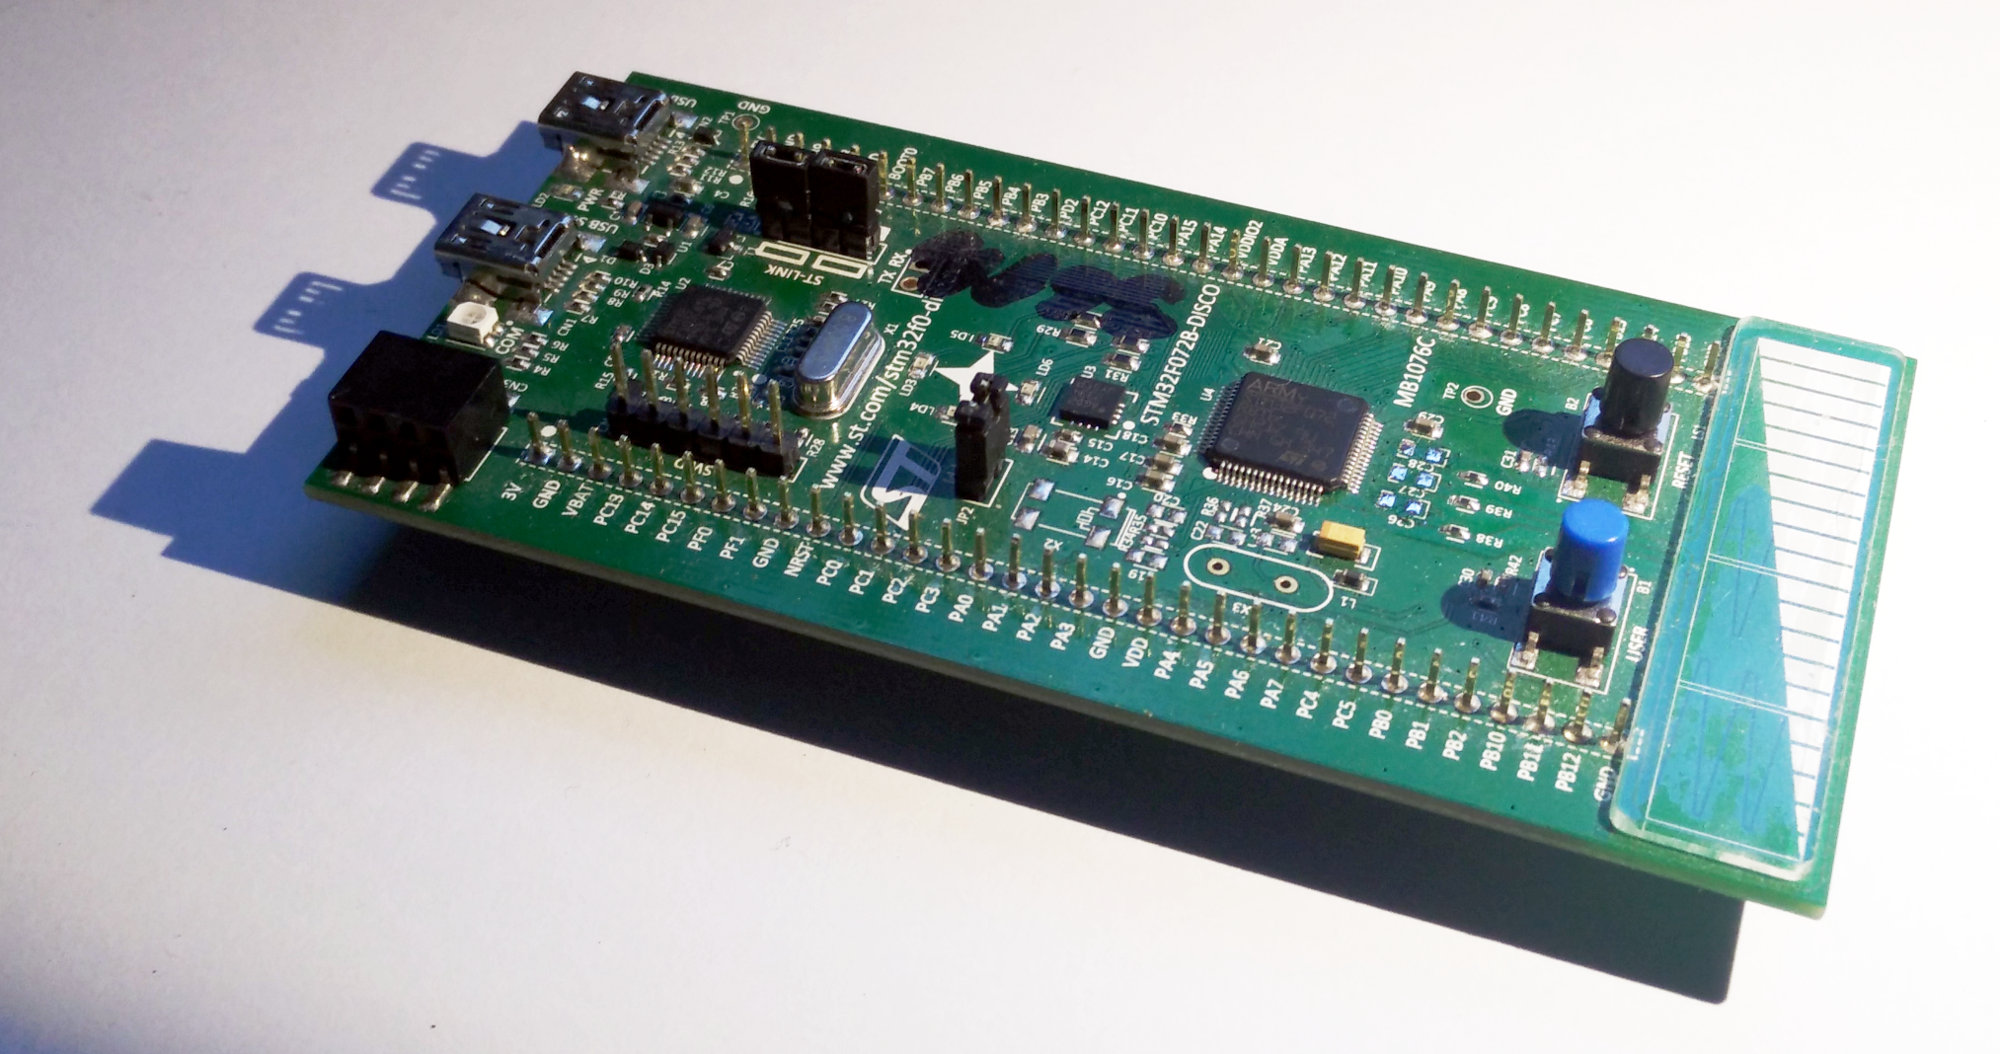
\includegraphics[width=0.9\textwidth] {img/disco072.jpg}
	\caption[A Discovery board with STM32F072]{\label{fig:discovery}A Discovery board with STM32F072 that can be used to run the GEX firmware}
\end{figure}


\begin{figure}
	\centering
	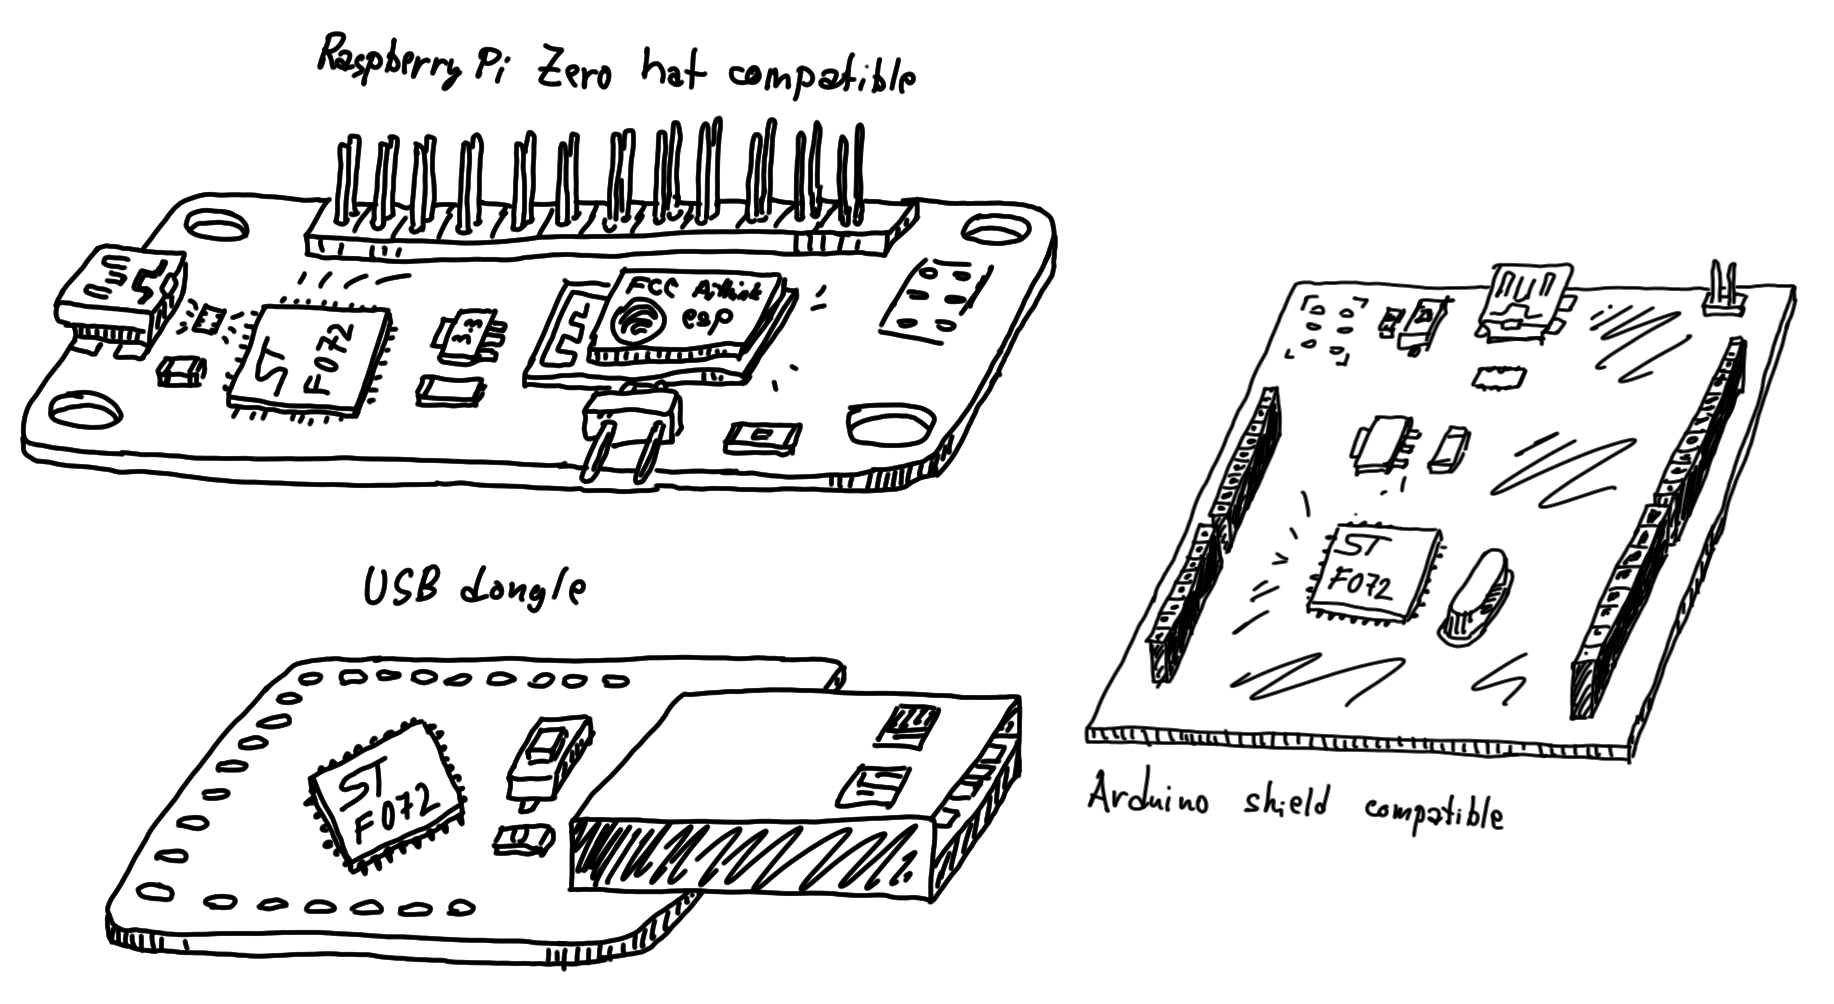
\includegraphics[width=\textwidth] {img/gex-ff-sketches.png}
	\caption[Form factor sketches]{\label{fig:ff-sketches}A sketch of three possible form factors for the GEX hardware prototype. Note the ESP8266 module which was considered as an option for wireless access but was eventually not used due to it's high current usage, unsuitable for battery operation.}
\end{figure}














